\documentclass[11pt]{article}
\usepackage[utf8]{inputenc}
\usepackage{algorithm}
\usepackage{algorithmic}
\usepackage{amsfonts}
\usepackage{amsmath}
\usepackage{amssymb}
\usepackage{amsthm}
\usepackage[english]{babel}
\usepackage{booktabs}
\usepackage[labelfont=bf, font=small]{caption}
\usepackage{chngcntr}
\usepackage{color, colortbl}
\usepackage{fancyhdr}
\usepackage{graphicx}
\usepackage[utf8]{inputenc}
\usepackage{listings}
\usepackage{microtype}
\usepackage[numbers]{natbib}
\usepackage{parskip}
\usepackage{subcaption}
\usepackage[most]{tcolorbox}
\usepackage{xcolor}

\usepackage[vcentering,dvips]{geometry}
\geometry{
    papersize={7in,9in},
    bottom=3pc,
    top=5pc,
    left=5pc,
    right=5pc,
    bmargin=4.5pc,
    footskip=18pt,
    headsep=25pt}


\usepackage[
  colorlinks=true,
  linkcolor=black,
  anchorcolor=black,
  citecolor=black,
  filecolor=black,
  menucolor=black,
  runcolor=black,
  urlcolor=black]{hyperref}

\setcounter{tocdepth}{2}

\definecolor{Gray}{gray}{0.9}
\newcommand{\dotscale}{0.7}

\theoremstyle{definition}
\renewcommand\qedsymbol{$\blacksquare$}
\newtheorem{example}{Example}[section]

% Section numbers in captions.
\counterwithin{figure}{section}
\counterwithin{table}{section}
\counterwithin{example}{section}
\counterwithin{algorithm}{section}

\fancyhf{}
\lhead{\leftmark}
\rhead{\thepage}
\pagestyle{fancy}

%% log-sum-exp
\DeclareMathOperator*{\LSE}{\textrm{LSE}}

%% Matrices
\newcommand{\mA}{{\bf A}}
\newcommand{\mB}{{\bf B}}
\newcommand{\mC}{{\bf C}}

%% Vectors
\newcommand{\vr}{{\bf r}}
\newcommand{\vu}{{\bf u}}
\newcommand{\vv}{{\bf v}}
\newcommand{\vx}{{\bf x}}
\newcommand{\vy}{{\bf y}}

%% Graphs
\newcommand{\gA}{\mathcal{A}}
\newcommand{\gB}{\mathcal{B}}
\newcommand{\gC}{\mathcal{C}}
\newcommand{\gE}{\mathcal{E}}
\newcommand{\gT}{\mathcal{T}}
\newcommand{\gU}{\mathcal{U}}
\newcommand{\gY}{\mathcal{Y}}
\newcommand{\gZ}{\mathcal{Z}}

%% Language
\renewcommand\L{\mathcal{L}}

%% <s> and </s> tokens
\newcommand{\sos}{\textrm{<s>}}
\newcommand{\eos}{\textrm{</s>}}


\title{An Introduction to Weighted Automata \\ in Machine Learning}
\author{Awni Hannun\footnote{
  Send correspondence to
  \href{mailto:awni.hannun@gmail.com}{awni.hannun@gmail.com}}}

\begin{document}

\maketitle

\begin{abstract}
    The goal of this work is to introduce the reader to weighted finite-state
    automata and their application to machine learning. I begin by motivating
    the use of automata in machine learning and proceed with an introduction to
    acceptors, transducers, and their associated properties. Many of the core
    operations of weighted automata are then described in detail. Following
    this, the work moves closer to the research frontier by explaining
    automatic differentiation and its use with weighted automata. The last
    section presents several extended examples to gain deeper familiarity with
    weighted automata, their operations, and applications to machine-learning.
\end{abstract}

\include{toc}
\section{Introduction}
\label{sec:introduction}

Relatively speaking, finite-state automata have a long history of application
in machine learning. The majority of these applications involve sequential
data.  For example, they are or have been used in speech recognition, machine
translation and other natural language tasks, and protein function analysis and
other tasks in computational biology.

However, the application of these data structures in machine learning is far
from main stream. In fact, their use likely decreased with the advent of
end-to-end deep learning. The recent development of frameworks for automatic
differentiation with automata suggests there may be renewed interest in the
application of automata to machine learning.

This tutorial introduces weighted automata and their operations. Once this
fundamental data structure is well understood, we then continue to build our
intuition by working through some extended examples.  I hope at minimum this
tutorial engenders an appreciation for the potential of automata in machine
learning. Ideally for some readers this tutorial will be a launching point for
the incorporation of automata in machine-learning research and applications.

However, before launching into the more technical content, let's start with
some broader perspectives in order to motivate the use of automata in machine
learning.

\subsection{Monolithic or Modular}

In the past, complex machine-learning systems, like those used in speech
recognition, involved many specialized hand-engineered components. The trend
is now for the opposite. Most machine-learning applications involve a single,
monolithic neural network. Both of these extremes have advantages and both have
disadvantages.

I believe a primary advantage of automata in machine learning is their
ability to harness the best of both worlds. Automata are capable of retaining
many if not all of the advantages of a multi-component, hand-engineered system
as well as those of a monolithic deep neural network. The next few paragraphs
explain some of these advantages and the regime to which they apply.

\paragraph{Modular:} One of the advantages of multi-component, hand-engineered
systems over monolithic neural networks is modularity. In traditional software
design modularity is usually a good thing. Modular systems are easier to
develop since part of the system can be changed without needing to change the
rest. In machine-learning systems, modularity is useful to avoid retraining the
entire system when only part of the model needs to be updated. Modularity can
also be useful when the individual modules can be reused. For example, speech
recognition systems are built from acoustic models and language models.
Acoustic models can be language agnostic and used for different languages.
Language models are general text based models which can be used in many
different tasks.

\paragraph{Compound errors:} A primary disadvantage of modular systems is that
errors compound. Each module is typically developed in isolation and hence
unaware of the types of errors made by the modules from which it receives
input. Monolithic systems on the other hand can be thought of as being
constructed from many sub-components all of which are jointly optimized towards
a single goal. These sub-components can learn to compensate for the mistakes
made by the others and in general work together more seamlessly.

\paragraph{Adaptable:} Modular systems are typically more adaptable than
monolithic systems. A machine-learning model which is tuned for one domain
usually won't work in another domain without retraining at least part of the
model on data from the new domain. Monolithic neural networks typically require
a lot of data and hence are difficult to adapt to new domains. Modular systems
must also be adapted. However, in some cases only one or a small subset of the
modules need be updated, making the adaptation problem simpler.

\paragraph{Learns from data:} One of the hallmarks of deep neural networks is
their ability to continue to learn and improve with larger data sets. Because
of the many assumptions hard-wired into more traditional modular systems, they
hit a performance ceiling much earlier as data set sizes increase. Retaining
the ability to learn when data is plentiful is a critical features of any
machine-learning system.

\paragraph{Prior knowledge:} On the other hand, one of the downsides of deep
neural networks is their need for large data sets to yield even decent
performance. Encoding prior knowledge into a model improves sample efficiency
and hence reduces the need for data. Encoding prior knowledge into a deep
neural networks is not easy. In some cases, encoding prior knowledge into a
neural network can be done, such as the translation invariance of convolutions.
However, in general, this is not so straightforward. Modular systems by their
very nature incorporate prior knowledge for a give task. Each module is
designed and built to solve a specific sub-task, usually with plenty of
potential for customization towards that task.

Modular and monolithic systems have complementary advantages with respect to
these four traits. Ideally we could construct machine-learning models which
retain the best of each. Automata-based modeling is one possibility which will
task us a step closer towards this goal.  However, to use automata to their
full potential we have to overcome a couple of challenges. The key is enabling
the use of weighted automata in training the model itself. This requires 1)
efficient implementations 2) easy to use frameworks which support automatic
differentiation.

\subsection{Advantages of Differentiable Automata}
\label{sec:advantages}

A key to unlocking the potential of automata in machine learning is enabling
their use during the training stage machine-learning models. All of the
operations I introduce later are differentiable with respect to the arc weights
of their input graphs. This means that weighted automata and the operations on
them can be used in a similar manner as tensors and their corresponding
operations are used in deep learning. Operations can be chained to form complex
computation graphs. Some of the weighted automata which are input to the
computation graph can have parameters which are learned. These parameters can
be optimized using back-propagation and gradient descent.

Automatic differentiation makes computing gradients for complex computation
graphs much simpler. Hence combining automatic differentiation with weighted
automata is important to enabling their use in training machine-learning
models.

Sophisticated machine-learning systems often separate the training and
inference stages of the algorithm. Multiple models are trained in isolation via
one code path. For prediction on new data, the individual models are combined
and rely on a different code path. The constraints of the two regimes (training
and inference) are such that separation from a modeling and software
perspective is often the best option. However, this is not without drawbacks.

First, from a pragmatic standpoint, having separate logic and code paths for
training and inference requires extra effort and usually results in bugs from
subtle mismatches between the two paths. Second, from a modeling standpoint,
optimizing individual models in isolation and then combining them is often
sub-optimal.

One of the benefits of combining automatic differentiation with weighted
automata is the potential to bring the training and inference stages closer
together. For example, speech recognition systems often uses hand-implemented
loss functions at training time. However, the decoder (used for inference)
brings together multiple models represented as graphs (lexicon, language model,
acoustic model, \emph{etc.}) in a completely different code path. By enabling
automatic differentiation with graphs, the decoding stage can also be used for
training.  This has the potential to both simplify and improve the performance
of the system.

Loss functions like Connectionist Temporal Classification, the Automatic
Segmentation criterion, and Lattice-free Maximum Mutual Information are
implemented with custom and highly optimized software. However, these loss
functions can all be implemented using graphs and (differentiable) operations
on graphs.

This separation of code from data, where graphs represent the data and
operations on graphs represent the code, has several benefits. First, the
separation simplifies the software. Second, the separation facilitates research
by making it easier to experiment with new ideas. Lastly, the separation
enables the optimization of graph operations to be more broadly shared.

\subsection{Comparison to Tensors}
\label{sec:comparison_to_tensors}

Modern deep learning is built upon the tensor data structure and the many
operations which take as input one or more tensors. Some of the more common
operations include matrix multiplication, 2-dimensional convolution, reduction
operations, and unary and binary operations.

Automata are an alternative data structure and the operations are quite
different in general. However, one can draw a loose analogy between the
operations on automata and those on tensors.
Table~\ref{tab:tensor_wfst_analogy} shows some of the common operations on
tensors and their analogous operations on automata. The analogy is quite loose,
but still useful at the very least as a mnemonic device and perhaps can help
build intuition for the various operations on graphs.

For example, superficially the formula for matrix multiplication and transducer
composition are quite similar. Assume we have three matrices such that $\mC = \mA
\mB$, then the $(i, j)$ element of $\mC$ is given by:
\begin{equation}
    C_{ij} = \sum_{k} A_{ik} B_{kj}
\end{equation}
Assume we have three transducers (graphs) where $\gC$ is the composition of
$\gA$ and $\gB$ , then the score of the path pair $(\vu, \vv)$ is given by:
\begin{equation}
    \mathcal{C}(\vu, \vv) = \LSE_{\vr} \mathcal{A}(\vu, \vr) + \mathcal{B}(\vr, \vv),
\end{equation}
where $\LSE$ is the \emph{log-sum-exp} operation.
%(we will describe composition
%in much more detail in section~\ref{sec:advanced_operations}).
Both operations take on the form of an accumulation over an inner variable of
values from each of the inputs. In matrix multiplication this is the shared
dimension of the matrices $\mA$ and $\mB$. In graph composition the inner
variable is the shared path $\vr$.

\begin{table}[ht]
    \renewcommand{\arraystretch}{1.4}
    \caption{The table shows loosely analogous operations between tensors and
    automata (acceptors and transducers).}
    \centering
    \begin{tabular}{l l l}
    \toprule
        Tensor & Automata \\
    \midrule
        Matrix multiplication, convolution & Intersect, compose \\
        \rowcolor{Gray} Reduction ops (sum, prod, \emph{etc.}) & Shortest distance (forward, Viterbi) \\
        Unary ops (power, negation, \emph{etc.})  & Unary ops (closure) \\
        \rowcolor{Gray} $n$-ary ops (addition, subtraction, \emph{etc.})  & $n$-ary ops (concatenation, union) \\
    \bottomrule
    \end{tabular}
    \label{tab:tensor_wfst_analogy}
\end{table}

A higher-level analogy to tensor-based deep learning can also be made. Modern
machine-learning frameworks like PyTorch and TensorFlow (and their ancestors
like Torch and Theano) were critical to the success of tensor-based deep
learning. These frameworks include support for automatic differentiation. They
also provide easy to use access to extremely efficient implementations of the
core operations. In the same way, automata-based machine learning should
benefit from frameworks with these features. We are just beginning to see new
developments in frameworks for automata-based machine learning including
GTN\footnote{I am a primary author of the GTN framework which is open source at
\url{https://github.com/gtn-org/gtn}} and K2\footnote{The K2 framework is the
successor of Kaldi and is open source at \url{https://github.com/k2-fsa/k2}}.
Perhaps these will encourage the use of automata in machine learning.

\subsection{History and Bibliographic Notes}

\citet{hopcroft2001introduction} provides an excellent introduction to
non-weighted automata. \citet{mohri2009weighted} gives a more formal and
general treatment of weighted automata and associated algorithms.

Weighted finite-state automata are commonly used in speech recognition, natural
language processing, optical character recognition, and other
applications~\citep{breuel2008ocropus, knight2009applications, mohri1997finite,
mohri2002weighted, mohri2008speech}. \citet{pereira1997} was an early
application of weighted automata to speech recognition, though before that
there were other applications in natural language
processing~\citep{pereira1994weighted, sproat1996stochastic}. The Graph
Transformer Networks of~\citet{bottou97}, a similar though more general
framework, were developed around the same time and applied to character
recognition in images.

The sequence criteria mentioned in section~\ref{sec:advantages}, namely
Connectionist Temporal Classification~\citep{graves2006}, the Automatic
Segmentation criterion~\citep{collobert2016wav2letter}, and Lattice-free
Maximum Mutual Information~\citep{povery2016purely} are most commonly used in
speech recognition. Section~\ref{sec:extended_examples} shows how to implement
a subset of these using weighted automata. \citet{hannun2017sequence} gives a
more detailed introduction to Connectionist Temporal Classification.


In terms of software, two of the better known libraries for operations on WFSTs
are OpenFST~\citep{mohri2000design} and its predecessor
FSM~\citep{allauzen2007openfst}. In section~\ref{sec:comparison_to_tensors} I
compared weighted automata to tensors. PyTorch~\citep{paszke2019pytorch} and
TensorFlow~\citep{abadi2016tensorflow} are two of the most used libraries for
tensor-based deep learning with automatic differentiation. These were based on
earlier frameworks including Torch~\citep{collobert2011torch7} and
Theano~\citep{bergstra2010theano}. Libraries which support automatic
differentiation with weighted automata have only recently been
developed~\citep{k2, hannun2020differentiable}.

\section{Acceptors and Transducers}
\label{sec:acceptors_transducers}

\subsection{Automata}
\label{sec:automata}

The broad class of graphs we are going to look at are finite-state automata.
These include deterministic finite-state automata (DFAs) and non-deterministic
finite-state automata (NFAs). More specifically we will consider a
generalization of DFAs and NFAs called weighted finite-state acceptors (WFSAs).
That's a mouthful, so I will just call them \emph{acceptors}. We will also
consider a further generalization of an acceptor called a \emph{transducer}
(weighted finite-state transducers or WFSTs). Figure~\ref{fig:wfsa_classes}
shows the relation between these three graphs; transducers, acceptors, and
automata. Transducers are the most expressive in terms of their
representational power, followed by acceptors followed by unweighted automata.

\begin{figure}
    \centering
    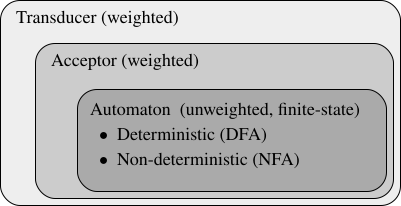
\includegraphics[width=0.7\linewidth]{figures/wfsa_classes}
    \caption{A hierarchy of automata classes from general to specific in terms
    of representation power. Weighted transducers can represent anything that
    weighted acceptors can represent. Weighted acceptors in turn can represent
    any unweighted finite-state automata.}
    \label{fig:wfsa_classes}
\end{figure}

Before we dive into acceptors and transducers, let's introduce some general
graph terminology that I will use throughout. In the following graph a
\emph{state} or \emph{node} is represented by a circle. The arrows represent
connections between two states. We usually refer to these as \emph{arcs} but
sometimes also \emph{edges}. The graph is directed since the connections
between states are unidirectional arrows. The arcs in a graph can have labels.
In figure~\ref{fig:simple_automata} the arc between states $0$ and $1$ has a
label of $a$. Similarly, the arc between states $1$ and $2$ has a label of $b$.
The graph is an example of a finite-state automata (FSA) or finite-state
machine (FSM), so called because it has a finite number of nodes.

\begin{figure}
    \centering
    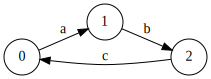
\includegraphics{figures/simple_automata}
    \caption{An example of a simple finite-state automata.}
    \label{fig:simple_automata}
 \end{figure}

An automata is deterministic if for each state and label pair there is only one
outgoing transition which matches that label. An automata is nondeterministic
if multiple transitions leaving a state have the same label. The graphs in
figure~\ref{fig:dfa_nfa} show an example of a deterministic and a
nondeterministic automata. In general, acceptors and transducers to can be
nondeterministic.

\begin{figure}
    \centering
    \begin{subfigure}[b]{0.48\textwidth}
        \includegraphics[scale=\dotscale]{figures/simple_dfa}
        \caption{Deterministic}
        \label{fig:simple_dfa}
    \end{subfigure}
    \begin{subfigure}[b]{0.48\textwidth}
        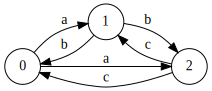
\includegraphics[scale=\dotscale]{figures/simple_nfa}
        \caption{Nondeterministic}
        \label{fig:simple_nfa}
    \end{subfigure}
    \caption{An example of a deterministic automata and a nondeterministic
    automata. The nondeterministic automata has two arcs leaving state $0$ both
    with label $a$ and two arcs leaving state $2$ both with the label $c$.}
    \label{fig:dfa_nfa}
\end{figure}

\subsection{Acceptors}

Let's start by constructing some very basic automata to get a feel for their
various properties.

The start state $s = 0$ has a bold circle around it. The accepting state $1$ is
represented with concentric circles. Each arc has a label and a corresponding
weight. So the first arc from state $0$ to state $1$ with the text $a/0$ means
the label is $a$ and the weight is $0$. The fact that there is only a single
label on each arc means this graph is an \emph{acceptor}. Since it has weights,
we say its a weighted acceptor. Since the number of states is finite, some
would call it a weighted finite-state acceptor or WFSA. Again, that's a
mouthful, so I'll just call these graphs acceptors.

\begin{figure}
    \centering
    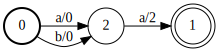
\includegraphics[scale=\dotscale]{figures/simple_fsa}
    \caption{An example of a simple acceptor. The label on each arc shows the
    input label and weight, so the $a/0$ represents a label of $a$ and a weight
    of $0$.}
    \label{fig:simple_fsa}
\end{figure}

An accepting path in the graph is a sequence of arcs which begin at a start
state and end in an accepting state. By concatenating the labels on an
accepting path, we get a string which is accepted by the graph. So the string
$aa$ is accepted by the graph by following the state sequence $0 \rightarrow 2
\rightarrow 1$. The string $ba$ is also accepted by the graph by following the
same state sequence but taking the arc with label $b$ when traversing from
state $0$ to state $1$. The language of the acceptor is the set of all strings
which are accepted by it. You may also encounter ``recognized'' used as a
synonym for ``accepted''. Let the variable $\gA$ represent the acceptor in
figure~\ref{fig:simple_fsa}. In general, I'll use uppercase script letters to
represent graphs. Let $\mathcal{L}(\gA)$ denote the language of $\gA$. In this
case $\mathcal{L}(\gA) = \{aa, ba\}$.

There are different ways to compute the weight of a string accepted by the
graph. The most common is to sum the weights of the arcs on the accepting path
for that string. For example the string $aa$ in the graph in
figure~\ref{fig:simple_fsa} has a weight of $0 + 2 = 2$. Another option would
be to multiply the weights. These two options correspond to interpreting the
weights as either log probabilities or probabilities. We'll have more to say
about this later.

The graph in figure~\ref{fig:multi_path} accepts the same sequence by multiple
paths.

\begin{figure}
    \centering
    \includegraphics[scale=\dotscale]{figures/multi_path}
    \caption{An acceptor which has multiple paths for the same sequence, $aa$.}
    \label{fig:multi_path}
\end{figure}

The string $aa$ is accepted along the state sequence $0 \rightarrow 2
\rightarrow 1$ and along the state sequence $0 \rightarrow 3 \rightarrow 1$. In
this case, to compute the score of $aa$ we need to consider both paths. Again
we have a couple of options here. The most common approach is to
\emph{log-sum-exp} the individual path scores. Again this corresponds to
interpreting the path scores as log probabilities. We'll use $\LSE(s_1, s_2)$
to denote the \emph{log-sum-exp} of the two scores $s_1$ and $s_2$:
\begin{equation}
\LSE(s_1, s_2) = \log \left( e^{s_1} + e^{s_2}\right).
\end{equation}
So the overall weight for the string $aa$ in the graph in
figure~\ref{fig:multi_path} is given by:
$$
\log \left(e^{0 + 2} + e^{1 + 3}\right) = 4.13.
$$

Acceptors can have multiple start states and multiple accept states. In the
graph in figure~\ref{fig:multi_start_accept}, the states $0$ and $1$ are both
start states, and the states $3$ and $4$ are both accept states.

\begin{figure}
    \centering
    \includegraphics[scale=\dotscale]{figures/multi_start_accept}
    \caption{An acceptor with multiple start states ($0$ and $1$) and multiple
    accept states ($3$ and $4$).}
    \label{fig:multi_start_accept}
\end{figure}

It turns out that allowing multiple start or accept states does not increase
the expressive power of the graph. With $\epsilon$ transitions (which we will
discuss soon), one can convert any graph with multiple start states and
multiple accept states into an equivalent graph with a single start state and a
single accept state.

Note also that start states can have incoming arcs (as in state $1$) and accept
states can have outgoing arcs, as in state $3$.

\begin{example}
Compute the score of the string $ab$ in figure~\ref{fig:multi_start_accept}.
\end{example}

\begin{proof}[\unskip\nopunct]
The two state sequences which accept the string $ab$ are the states $0
\rightarrow 2 \rightarrow 3$ and $1 \rightarrow 3 \rightarrow 4$. The overall
score is given by:
$$
\log (e^{1 + 3} + e^{1 + 2}) = 4.31.
$$
\end{proof}

Graphs can also have self-loops and cycles. For example, the graph in
figure~\ref{fig:fsa_loops} has a self-loop on the state $0$ and a cycle
following the state sequence $0 \rightarrow 1 \rightarrow 2 \rightarrow 0$.

\begin{figure}
    \centering
    \includegraphics[scale=\dotscale]{figures/fsa_loops}
    \caption{A graph with a self-loop on the state $0$ and a cycle from $0
    \rightarrow 1 \rightarrow 2 \rightarrow 0$.}
    \label{fig:fsa_loops}
\end{figure}

The language of a graph with cycles and self-loops contains infinitely many
strings.  For example, the language of the graph in figure~\ref{fig:fsa_loops}
includes any string that starts with zero or more $a$s and ends in $bb$. As a
regular expression we write this as $a^*bb$ where the $^*$ denotes zero or more
$a$s.

The $\epsilon$ symbols has a special meaning when it is the label on an arc.
Any arc with an $\epsilon$ label can be traversed without consuming an input
token in the string. So the graph in figure~\ref{fig:fsa_epsilon} accepts the
string $ab$, but it also accepts the string $b$ because we can traverse from
state $0$ to state $1$ without consuming an input.

\begin{figure}
    \centering
    \includegraphics[scale=\dotscale]{figures/fsa_epsilon}
    \caption{An acceptor with an $\epsilon$ transition on the second arc
    between state $0$ and $1$.}
    \label{fig:fsa_epsilon}
\end{figure}

As it turns out, any graph with $\epsilon$-transitions can be converted to an
equivalent graph without $\epsilon$ transitions. However, this usually comes at
a large cost in the size of the graph. Complex languages can be represented by
much more compact graphs with the use of $\epsilon$-transitions.

\begin{example}
Convert the graph in figure~\ref{fig:multi_start_accept} which has multiple
start and accept states to an equivalent graph with only a single start and
accept state using $\epsilon$ transitions.
\end{example}

\begin{proof}[\unskip\nopunct]
The graph in figure~\ref{fig:epsilon_start_accept} is the equivalent graph
with a single start state and a single accept state.

\begin{figure}
    \centering
    \includegraphics[scale=\dotscale]{figures/epsilon_start_accept}
    \caption{The equivalent graph using only a single start state and accept
    state to the graph in figure~\ref{fig:multi_start_accept} which has
    multiple start and accept states.}
    \label{fig:epsilon_start_accept}
\end{figure}

The construction works by creating a new start state and connecting it to the
old start states with $\epsilon$ transitions with a weight of $0$. The old
start nodes are regular internal nodes in this new graph. Similarly the old
accept states are now regular states and they connect to the new accept state
with $\epsilon$ transitions with a weight of $0$.
\end{proof}

\subsection{Transducers}

A \emph{transducer} maps input strings to output strings. Transducers are a
generalization of an acceptors. Every acceptor is a transducer, but not every
transducer is an acceptor. Let's look at a few example transducers to
understand how they work.

The arc labels distinguish an acceptor from a transducer. A transducer has both
an input and output arc label. The arc labels are of the form $a\!:\!x/0$ where
$a$ is the input label $x$ is the output label and $0$ is the weight. An
acceptor can be represented as a transducer where the input and output labels
on every arc are identical.

\begin{figure}
    \centering
    \includegraphics[scale=\dotscale]{figures/simple_fst}
    \caption{An example of a simple transducer. The label on each arc shows the
    input label, the output label, and the weight. So $a\!:\!x/0$ represents an
    input label of $a$, and output label of $x$, and a weight of $0$.}
    \label{fig:simple_fst}
\end{figure}

Instead of saying that a transducer accepts a given string, we say that it
\emph{transduces} one string to another. The graph in
figure~\ref{fig:simple_fst} transduces the string $ab$ to the string $xz$ and
the string $bb$ to the string $yz$. The weights of a transduced pair is
computed in the same way as in an acceptor. The scores of the individual arcs
on the path are summed. The path scores are combined with \emph{log-sum-exp}.
So the weight of the transduced pair $(ab, xz)$ in the graph in
figure~\ref{fig:simple_fst} is $0+3 = 3$.

We have to generalize concept of the language from an acceptor to a transducer.
I'll call this generalization the transduced set. Since it will always be clear
from context if the graph is an acceptor or transducer, I'll use the same
symbol $\mathcal{L}$ to represent the transduced set. If $\gT$ is a transducer,
then $\mathcal{L}(\gT)$ is the set of pairs of strings transduced by $\gT$.
More formally, a pair of strings $(\vx, \vy) \in \mathcal{L}(\gT)$ if $\gT$
transduces $\vx$ to $\vy$.

\begin{example}
Compute the score of the transduced pair $(aab, zyy)$ in the graph in
figure~\ref{fig:fst_example_score}.
\end{example}

\begin{proof}[\unskip\nopunct]
\begin{figure}
    \centering
    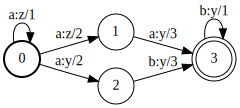
\includegraphics[scale=\dotscale]{figures/fst_example_score}
    \caption{An example transducer in which the sequence $aab$ is transduced to
    the sequence $zyy$ on multiple paths.}
    \label{fig:fst_example_score}
\end{figure}

The two paths which transduce $aab$ to $zyy$ are following the state sequence
$0 \rightarrow 1 \rightarrow 3 \rightarrow 3$ and $0 \rightarrow 0 \rightarrow
2 \rightarrow 3$. The score of the first path is $6$ and the score of the
second path is $6$. So the overall score is:
$$
\log \left(e^6 + e^6\right) = 6.69.
$$
\end{proof}

Transducers can also have $\epsilon$ transitions. The $\epsilon$ can be either
the input label on an arc, the output label on an arc, or both. When the
$\epsilon$ is the input label on an arc, it means we can traverse that arc
without consuming an input token, but we still output the arc's corresponding
output label. When the $\epsilon$ is the output label, the opposite is true.
The input is consumed but no output is produced. And when the $\epsilon$ is
both the input and the output label, the arc can be traversed without consuming
an input or producing an output.

\begin{figure}
    \centering
    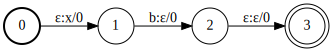
\includegraphics[scale=\dotscale]{figures/fst_epsilon}
    \caption{A transducer with $\epsilon$ transitions. The $\epsilon$ can be
    just the input label, just the output label, or both the input and output
    label.}
    \label{fig:fst_epsilon}
\end{figure}

In the graph in figure~\ref{fig:fst_epsilon}, the string $b$ gets transduced to
the string $x$. On the first arc between states $0$ and $1$, we output an $x$
without consuming any token. On the second arc between states $1$ and $2$, a
$b$ is consumed without outputting any new token. Finally, on the arc between
states $2$ and $3$ we neither consume nor output a token.

\section{Basic Operations}
\label{sec:basic_operations}

\section{Advanced Operations}
\label{sec:advanced_operations}

\documentclass[main.tex]{subfiles}
\begin{document}

\section{Differentiable Automata}
\label{sec:differentiable_automata}

\end{document}

\section{Extended Examples}
\label{sec:extended_examples}

\include{bibliography}

\end{document}
